
\item A boy is pushing a ring of mass 2 kg and radius 0.5 m with a stick as shown in the figure. The stick applies a force of 2 N on the ring and rolls it without slipping with an acceleration of \(0.3 \, \text{m/s}^2\). The coefficient of friction between the ground and the ring is large enough that rolling always occurs and the coefficient of friction between the stick and the ring is \(\frac{P}{10}\). The value of P is \underline{\hspace{2.5cm}}.
    \begin{center}
        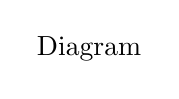
\begin{tikzpicture}
            % Since the diagram is complex and cannot be recreated entirely with LaTeX commands without more details, a placeholder is left.
            \node at (0, 0) {Diagram}; % Replace this with the actual TikZ commands to draw the diagram.
        \end{tikzpicture}
    \end{center}
